\section{高速化に対する弾性の影響}
\label{sec:elasticity-discussion}

\subsection{高速化度合と応力比の関係}
第\ref{sec:viscosity}章で示した通り,超音波照射による球の高速化の要因として粘性による影響では説明が十分にできない.そこで,本章では先行研究\cite{ref:8}で示唆された弾性影響を考える.

第\ref{sec:elasticity}節にて,貯蔵弾性率$G'$,損失弾性率$G''$と応力$\tau$の関係を示した.また,弾性と粘性の支配要素が変わる応力$\tau_\text{0}$も示した.この応力$\tau_\text{0}$と落下する球によって生じる応力$\tau_\text{U}$(式(\ref{eq:tauU}))の比$\tau_\text{U}/\tau_\text{0}$を考える.この比が1より大きいと粘性影響が,1より小さいと弾性影響が大きいとみなす.

応力比と終端速度の関係をFig\ref{fig:elastcity}(a)に示す.終端速度が高くなると,応力比が増加した.式(\ref{eq:tauU})において,擬塑性流体($0<n<1$)では,終端速度が高くなると$\tau_\text{U}$が大きくなるためである.終端速度が高くなると粘性影響の寄与が示唆される.

式(\ref{eq:muU}),(\ref{eq:muABL}),(\ref{eq:Udiff})より,高速化度合い$U_\text{on}/U_\text{off}$には以下の比例関係が成り立つ.
\begin{eqnarray}
    \frac{U_\text{on}}{U_\text{off}} \sim U_\text{off}^{n-1} \left(\frac{1}{u}\right)^{n-1} \left(\frac{\delta}{a}\right)^n .
    \label{eq:UTdiff_UT}
\end{eqnarray}
擬塑性流体($0<n<1$)では,終端速度$U_\text{off}$の指数は負となり,終端速度が遅い場合,高速化がより顕著に現れると考えられる.高速化度合いと終端速度の関係をFig\ref{fig:elastcity}(b)に示す.終端速度が低くなると高速化度合が大きくなったが,高速化度合いのばらつきは大きい.ばらつきが大きいのは,終端速度だけでなく,音響境界層の影響を受けるためと考えられる.

応力比と高速化度合いの関係をFig\ref{fig:elastcity}(c),(d)に示す.Fig\ref{fig:elastcity}(c)は全ての実験結果を,Fig\ref{fig:elastcity}(d)はPAA濃度0.2wt.\%,岩室\cite{ref:8}以外の実験結果を示す.先行研究\cite{ref:8}の実験結果を含めた場合,明瞭な相関が見られない.球の落下による応力は超音波照射していない状態における終端速度にて定義している.一方で,先行研究\cite{ref:8}は,照射する超音波周波数,平均圧力振幅,球径をパラメータとしている.このため,超音波周波数や平均圧力振幅を考慮していない落下球による応力比による整理では不十分であると考えられる.今回の実験結果では応力比1近傍にて高速化が顕著に現れた.式(\ref{eq:tauU}),(\ref{eq:UTdiff_UT})より,終端速度が低くなると球の落下による応力が小さくなり,高速化度合が大きくなる.しかし,応力比が1より小さくなると,高速化が抑制されていた.これは,粘性ではなく弾性影響が強まるためと考えられる.

\begin{figure}[H]
    \centering
    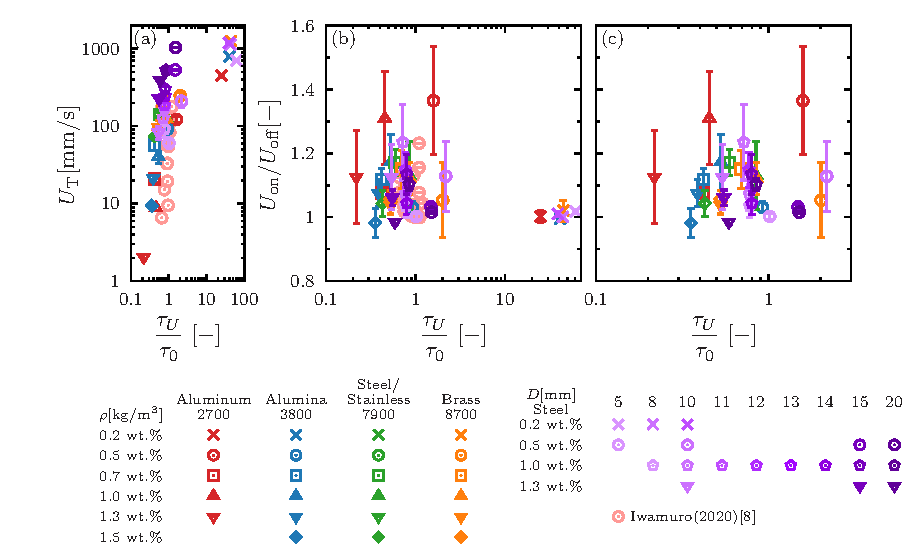
\includegraphics[width=1.0\textwidth]{5-Results/elastcity.eps}
    \caption{Relationship between terminal velocity and (a)elasticity ratio $\tau_\text{U}/\tau_\text{0}$, (b)velocity ratio, elasticity ratio $\tau_\text{U}/\tau_\text{0}$ and velocity ratio by (c)all experiment, (d)without 0.2wt.\% PAA solution.}
    \label{fig:elastcity}
\end{figure}

\subsection{高速化に対する粘度比・応力比の影響}
第\ref{sec:viscosity}章において,高速化度合いと粘度比の関係を示した.また,前節で超音波照射による落下速度の高速化度合いと応力比の関係を示した.本節にて,高速化度合いに対する粘度比,応力比両方との関係を考える.これにより,超音波照射による球の高速化に対する粘弾性影響を検討する.応力比と粘度比と音響境界層厚さを球の半径で規格化した値の積の関係を,Fig\ref{fig:elastcityColor}に示す.カラーバーは高速化度合を表す.横軸の値が大きいほど,応力比は小さくなる.これは,粘度比が大きくなると,弾性影響が強くなることを示している.横軸の値が0.01近傍では,高速化度合いが1.03以下であり高速化がほぼ見られなかった.これは,粘度が小さいためであると考えられる.粘度比が大きいと応力比は小さくなる.Fig\ref{fig:viscosity_ratio}より,粘度比0.2近傍,応力比1近傍にて高速化度合は1.15以上となり,顕著である.その後,粘度比が0.2以上では,応力比は1以下となる.このような条件では,高速化度合は1.05程度であり,高速化が弱くなった.そして,粘度比が1以上において,高速化度合は1.08程度であり,先述の条件よりも高速化は見られた.この条件では弾性が支配的ではあるが,粘度比が大きいため高速化が促進されたと示唆される.以上より,超音波照射による球の落下の高速化に関して,弾性による影響現れると示唆される.

\begin{figure}[H]
    \centering
    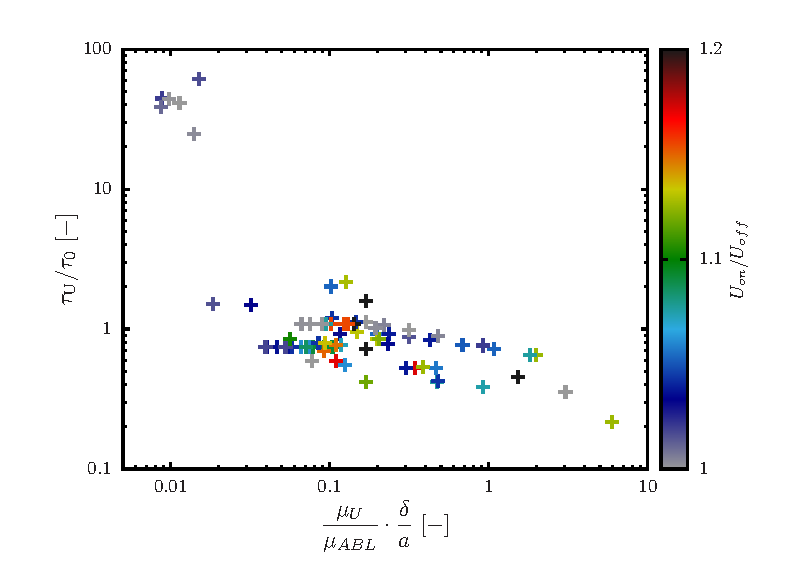
\includegraphics[width=0.9\textwidth]{5-Results/elastcity_color.eps}
    \caption{Relationship between velocity ratio and the inverse of the viscosity ratio multiplied by the thickness, elasticity ratio $\tau_\text{U}/\tau_\text{0}$.}
    \label{fig:elastcityColor}
\end{figure}
